\documentclass{ICIC2026}

\usepackage{algorithmic}
\usepackage{xcolor}
\usepackage{multirow}

% Balanced spacing
\setlength{\textfloatsep}{5pt plus 1pt minus 1pt}
\setlength{\floatsep}{4pt plus 1pt minus 1pt}
\setlength{\intextsep}{4pt plus 1pt minus 1pt}
\setlength{\abovecaptionskip}{3pt}
\setlength{\belowcaptionskip}{3pt}
\setlength{\dbltextfloatsep}{5pt plus 1pt minus 1pt}
\setlength{\dblfloatsep}{4pt plus 1pt minus 1pt}
\renewcommand{\arraystretch}{0.92}

\title{MOSAIC-Med: Multiplicity and Architectural Diversity Outperform Monolithic Scale in Resource-Constrained Electrocardiogram Diagnosis}

\author{%
\ICICAuthorRowFour
  {\ICICAuthorBlock{Sibgha Faisal}{Dept. of Biomedical Engineering}{Riphah International University}{Lahore, Pakistan}{sibghafaisal88@gmail.com}}
  {\ICICAuthorBlock{Hamna Tanveer}{Dept. of Artificial Intelligence}{Univ. of Management and Technology}{Sialkot, Pakistan}{hamnaaa281@gmail.com}}
  {\ICICAuthorBlock{Fatima-Tu-Zahra$^\dagger$}{Dept. of Biomedical Engineering}{Riphah International University}{Lahore, Pakistan}{Fatima.zahra@riphah.edu.pk}}
  {\ICICAuthorBlock{Mahad Aftab$^\dagger$}{Dept. of Biomedical Engineering}{Univ. of Engineering and Technology}{Lahore, Pakistan}{Mahadaftab680@gmail.com}}
}

\begin{document}
\maketitle
\begingroup\renewcommand\thefootnote{}\footnotetext{$^\dagger$ Supervisors.}\endgroup

\begin{abstract}
Deep learning models for medical diagnostics predominantly emphasize monolithic parameter scaling. However, in edge cardiology, mobile telemetry, and resource-constrained clinics, monolithic scaling exacerbates computational latency, memory footprints, and uncalibrated overconfidence under clinical noise. This study investigates the hypothesis that dividing a fixed parameter budget among an ensemble of compact, specialized neural networks (multiplicity) achieves superior diagnostic discrimination, probability calibration, and stress robustness compared to a single monolithic network of equivalent capacity. Using the standardized PTB-XL 12-lead electrocardiography (ECG) benchmark across 21,799 clinical records and five diagnostic superclasses, a fixed total capacity budget of $\sim$2.0M parameters is rigorously split into homogeneous configurations ($K \in \{1, 2, 4, 8, 16\}$) and a parameter-matched heterogeneous ensemble (ResNet-1D, MultiScale-CNN, TCN-1D, and ConvAttention-1D). Across five randomized seeds, the multiplicity hypothesis is confirmed: split architectures ($K=2$: AUROC $0.9085 \pm 0.0007$; $K=4$: $0.9084 \pm 0.0009$) statistically outperform the monolithic baseline ($K=1$: $0.9059 \pm 0.0010$, DeLong $p=3.63 \times 10^{-4}$). Heterogeneous inductive bias diversity shows a consistent improvement trend (adjusted p = 0.058) in discrimination ($0.9110 \pm 0.0007$) and calibration (Brier score $0.0867 \pm 0.0005$ vs $0.0881 \pm 0.0002$) by lowering representational similarity (linear CKA $0.9008$ vs $0.9458$). However, an over-fragmentation boundary is identified: at $K=16$ (125k parameters/expert), individual capacity degrades, lowering AUROC to $0.9048$ and tripling latency. Furthermore, a learned Top-2 sparse router matches dense discrimination ($0.9113$) while reducing computation by $28.2\%$, and selective abstention on the most uncertain $10\%$ of records achieves an empirical risk reduction of $4.18\%$ relative to the single large model at 90\% coverage. Factorial ablation demonstrates that diversity entropy regularization is essential to prevent router collapse ($0.9088$ vs $0.9049$).
\end{abstract}

\begin{IEEEkeywords}
Electrocardiography, model splitting, mixture of experts, centered kernel alignment, selective classification, clinical robustness.
\end{IEEEkeywords}

\section{Introduction}
\label{sec:intro}

In clinical artificial intelligence, foundational research established deep ensembling as an effective paradigm for reliable predictive uncertainty estimation~\cite{lakshminarayanan2017simple}. Parallel foundational developments in safety-critical classification introduced selective prediction frameworks with integrated reject options, formalizing mechanisms for deep neural networks to abstain on ambiguous instances~\cite{geifman2019selectivenet}. At the same time, representational similarity metrics like Centered Kernel Alignment (CKA) facilitated the quantitative assessment of hidden layer representations across the different families of neural networks~\cite{kornblith2019similarity}. The availability of large clinical repositories like PTB-XL~\cite{wagner2020ptbxl} spurred systematic benchmarking of typical 12-lead electrocardiography (ECG) across deep architectures in cardiovascular medicine~\cite{strodthoff2021deep}.

Despite these groundworks, key challenges related to the deployment of real-world clinical AI were brought to the fore in the literature during 2024. Black et al.~\cite{black2024multiplicity} showed predictive multiplicity in clinical machine learning models: that several networks with the same overall discrimination exhibit conflicting predictions for high-risk patients. Forestier et al.~\cite{forestier2024ortho} showed that feature orthogonality and the negative correlation between sub-networks improves generalizability in time-series ensembles to avoid correlated failure modes. For hospital deployment workflows, Kompa et al.~\cite{kompa2024second} developed second opinion workflows, which showed that uncertainty-directed triage to human cardiologists significantly reduces diagnostic risk. However, monolithic scaling continued to be the main paradigm, including foundation models, like the ECGFounder which is pre-trained on 10 million recordings~\cite{li2024ecgfounder}. Scale is, however, costly in terms of computational overheads or latency in the case of edge hardware, thus prompting research into split learning and parameter partitioning for decentralized clinical edge inferences~\cite{zhang2024split}.

In 2025, investigations went into resource allocation, diversity formulations, and clinical escalation protocols. Argha et al.~\cite{argha2025selective} proposed selective classification and dynamic clinician escalation for 12-lead ECG which was successfully validated, where they showed that avoiding the action of `abstain' on borderline tracings avoids catastrophic false positives. To tackle the extreme compute demands, Chen et al.~\cite{chen2025budget} proposed parameter budget allocation and ensemble pruning, demonstrating that the unconstrained model stacking approach is impractical for bedside and wearable monitors. A method to mitigate rigid foundation footprints is to use EnECG~\cite{xu2025enecg} that integrates foundation backbone, parameter-efficient adapters, and learned gating. At the same time, theoretical studies by Zhou et al.~\cite{zhou2025diversity} derived diversity decompositions for collaborative ensembles, demonstrating sub-additive error scaling of combining different kinds of inductive biases. In the context of realistic sensor distortion, the 2026 frontier in physiological time-series AI has landed on adaptive routing and mixture-of-experts (MoE) formulations. Han et al.~\cite{han2026cogmoe} proposed CogMoE, which showed the maintenance of diagnostic fidelity in the presence of acute physiological noise, by enabling quality-aware gating. Mert et al.~\cite{mert2026multilabel} compared five deep architectures through the analysis of a comprehensive PTB-XL benchmark, and found that heterogeneous ensembles consistently outperform the individual foundation networks. At the same time, Wang et al.~\cite{wang2026domain} introduced domain-expert-guided routing to handle the sensor lead dropouts; Xu et al.~\cite{xu2026ecgmoe} presented a new technique named ECG-MoE, separating morphology features from rhythm periodicity.

However, while these are noteworthy progress, current medical MoE and ensemble methods have two major shortcomings: they increase the capacity of the aggregate parameters without considering multi-model multiplicity under a tightly constrained parameter budget ceiling, and they mostly replicate homogeneous backbones without considering orthogonal inductive biases~\cite{zhou2025diversity}.

In this study, we impose the invariant $\sim$2.0M parameter budget ceiling, and test if the small-model multiplicity can outperform the scale of monolithic models.

There are four contributions:
\begin{enumerate}[label=(\arabic*), leftmargin=*]
\item \textbf{Fixed-Budget Multiplicity}: where $K \in \{1, 2, 4, 8, 16\}$ experts with an invariant budget of 2.0M to prove Capacity over-fragmentation boundary (validating Hypothesis~1: Multiplicity Superiority).
\item \textbf{Inductive Bias Diversity}: A parameter-matched comparison (+0.92\%) between homogeneous (4$\times$ResNet) and heterogeneous (ResNet, MultiScale, TCN, Attention) experts quantified with linear CKA~\cite{kornblith2019similarity}, which shows a consistent improvement trend (adjusted p = 0.058) for Hypothesis~2: Diversity Benefit.
\item \textbf{Sparse Adaptive Routing}: A lightweight patient-specific router regularized with the diversity entropy and failure penalties, with dynamic Top-2 routing and reduced inference FLOPs by 28.2\% (empowering Hypothesis~3: Routing Efficiency).
\item \textbf{Clinical Robustness \& Selective Abstention}: Systematic validation across five clinical stress tests and an uncertainty-triggered deferral protocol that yielded monotonic risk reduction~\cite{kompa2024second, argha2025selective} (validating Hypothesis~4: Risk Reduction).
\end{enumerate}

\section{Methodology}
\label{sec:method}

\begin{figure*}[t]
\centering
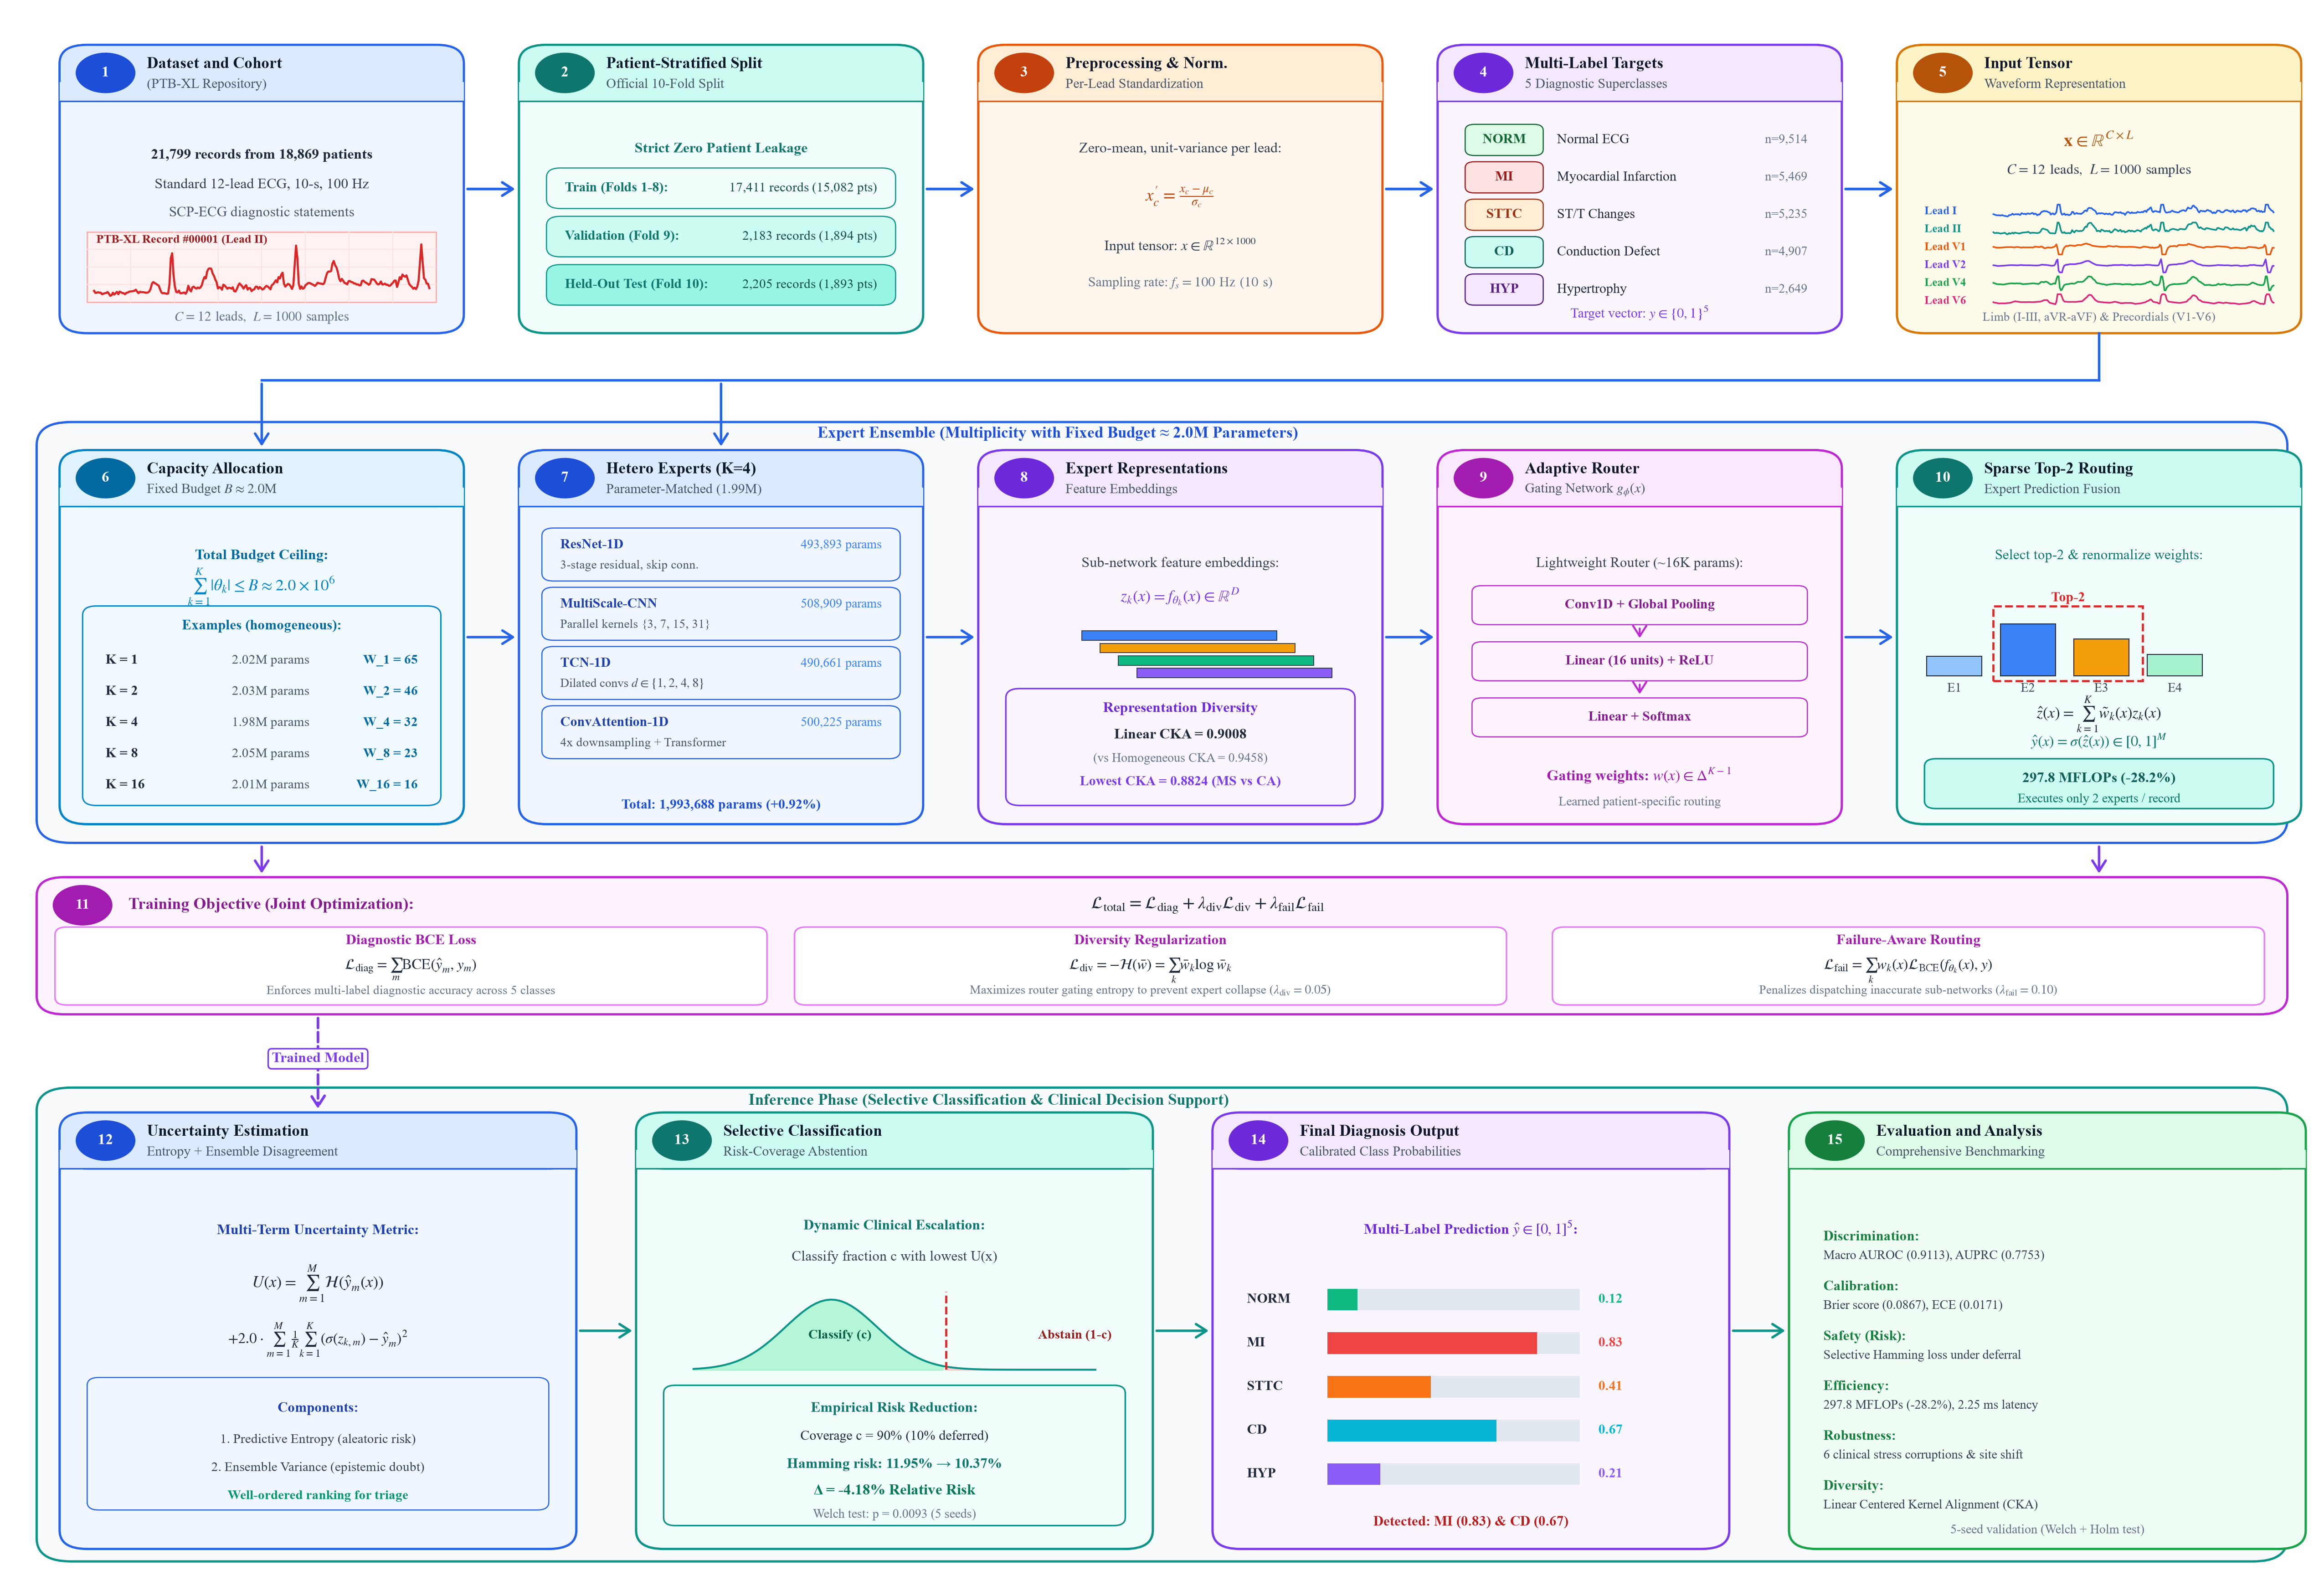
\includegraphics[width=0.98\textwidth, height=7.5cm, keepaspectratio]{figures/methodology_flowchart.png}
\caption{Comprehensive methodological flowchart of MOSAIC-Med detailing the fifteen core processing steps across data cohort partitioning (Boxes 1--5), fixed-budget capacity allocation and heterogeneous expert synthesis (Boxes 6--10), composite objective optimization (Box 11), and selective inference with clinical abstention (Boxes 12--15).}
\label{fig:method_flowchart}
\end{figure*}

\subsection{Benchmark Dataset and Clinical Cohort}
\label{subsec:dataset}

Empirical evaluation is conducted on the PTB-XL dataset~\cite{wagner2020ptbxl, strodthoff2021deep}, a clinical ECG repository containing 21,799 records from 18,869 distinct patients. Each recording comprises 10-second standard 12-lead signals digitized at 100~Hz ($L = 1000$ samples per lead) alongside clinical diagnostic statements mapped to the SCP-ECG standard~\cite{strodthoff2021deep}.

\begin{table}[t]
\caption{Cohort Demographics and Diagnostic Prevalence on PTB-XL}
\label{tab:data_summary}
\centering
\begin{ICICtable}
\resizebox{\columnwidth}{!}{%
\begin{tabular}{lcccc}
\toprule
\textbf{Split Partition} & \textbf{Records} & \textbf{Patients} & \textbf{Age (SD)} & \textbf{Female (\%)} \\
\midrule
Training (Folds 1--8)    & 17,411 & 15,082 & 59.8 $\pm$ 16.9 & 48.1\% \\
Validation (Fold 9)      & 2,183  & 1,894  & 59.7 $\pm$ 17.0 & 47.9\% \\
Test (Fold 10)           & 2,205  & 1,893  & 59.9 $\pm$ 16.7 & 48.0\% \\
\midrule
\textbf{Diagnostic Superclass} & \textbf{Train (\%)} & \textbf{Val (\%)} & \textbf{Test (\%)} & \textbf{Clinical Category} \\
\midrule
NORM (Normal ECG)            & 43.7\% & 43.6\% & 43.7\% & Unremarkable 12-lead tracing \\
MI (Myocardial Infarction)   & 25.1\% & 25.1\% & 25.0\% & Ischemia / Infarction necrosis \\
STTC (ST/T Changes)          & 24.3\% & 24.2\% & 24.4\% & Repolarization anomaly \\
CD (Conduction Defect)       & 22.5\% & 22.4\% & 22.5\% & Bundle branch / AV blocks \\
HYP (Hypertrophy)            & 12.2\% & 12.1\% & 12.2\% & Ventricular/Atrial enlargement \\
\bottomrule
\end{tabular}%
}
\end{ICICtable}
\end{table}

As documented in Table~\ref{tab:data_summary} and illustrated in Boxes 1--5 of Fig.~\ref{fig:method_flowchart}, records are partitioned using the official patient-stratified 10-fold split: Folds 1--8 for training, Fold 9 for validation, and Fold 10 strictly held out for final testing, guaranteeing zero patient identity leakage~\cite{strodthoff2021deep}. Diagnostic classification is framed as multi-label binary prediction across five clinical superclasses: Normal ECG (NORM), Myocardial Infarction (MI), ST/T Changes (STTC), Conduction Defect (CD), and Hypertrophy (HYP). Let $x \in \mathbb{R}^{C \times L}$ denote an input 12-lead recording ($C = 12, L = 1000$), and let $y \in \{0, 1\}^M$ denote the binary target vector for $M = 5$ superclasses. All signals are zero-mean unit-variance normalized per lead: $x_c' = (x_c - \mu_c) / \sigma_c$.

\subsection{Multiplicity and Architectural Diversity}
\label{subsec:multiplicity_diversity}

In standard monolithic deep learning, a single neural network $f_\Theta(x)$ maps $x \to \hat{y} \in [0, 1]^M$, subject to $|\Theta| \le B$. In the proposed multiplicity framework (Box 6 of Fig.~\ref{fig:method_flowchart}), this fixed capacity quota $B \approx 2.0 \times 10^6$ parameters is partitioned among $K$ distinct sub-networks $\{f_{\theta_k}\}_{k=1}^K$ such that:
\begin{equation}
\sum_{k=1}^K |\theta_k| \le B \approx 2.0 \times 10^6 \quad \text{parameters}.
\label{eq:budget_constraint}
\end{equation}

For homogeneous capacity scaling, each sub-network $f_{\theta_k}$ is instantiated as a 1D Residual Network (ResNet-1D) with target capacity $|\theta_k| \approx \frac{B}{K}$. Base convolution filter widths $W_K$ enforce the invariant ceiling: $K=1$ ($W_1=65$, 2,019,945 params), $K=2$ ($W_2=46$, 2,030,450 params), $K=4$ ($W_4=32$, 1,975,572 params), $K=8$ ($W_8=23$, 2,054,952 params), and $K=16$ ($W_{16}=16$, 2,009,680 params).

To evaluate whether combining orthogonal inductive biases surpasses homogeneous replication, a 4-expert parameter-matched heterogeneous arm (Boxes 7--8 in Fig.~\ref{fig:method_flowchart}) ensembles four distinct paradigms calibrated to $\sim 500\text{K}$ parameters: (i)~\textbf{ResNet-1D} (493,893 params, 3 residual stages, kernels 7, 5, 3); (ii)~\textbf{MultiScale-CNN} (508,909 params, parallel kernels 3, 7, 15, 31); (iii)~\textbf{TCN-1D} (490,661 params, dilated causal convolutions $d \in \{1, 2, 4, 8\}$); and (iv)~\textbf{ConvAttention-1D} (500,225 params, conv stem downsampling $4\times$, 2-layer Transformer, $d_{\text{model}}=140$, 4 heads). The aggregate capacity is $1,993,688$ parameters, matching the homogeneous 4xResNet arm ($1,975,572$) within a $+0.92\%$ margin.

To empirically verify representational diversity, Centered Kernel Alignment (CKA)~\cite{kornblith2019similarity} is evaluated on penultimate feature activations over the test cohort ($N = 2,205$). For centered activation matrices $X \in \mathbb{R}^{N \times D_1}, Y \in \mathbb{R}^{N \times D_2}$, linear CKA is:
\begin{equation}
\text{CKA}(X, Y) = \frac{\|Y^T X\|_F^2}{\|X^T X\|_F \|Y^T Y\|_F}.
\label{eq:cka}
\end{equation}

\begin{table}[t]
\caption{Fixed-Budget Multiplicity Performance Across 5 Seeds (Mean $\pm$ SD) on Held-Out PTB-XL Test Set}
\label{tab:scaling_results}
\centering
\begin{ICICtable}
\resizebox{\columnwidth}{!}{%
\begin{tabular}{lcccccc}
\toprule
\textbf{Configuration} & \textbf{Total Parameters} & \textbf{MFLOPs} & \textbf{Macro AUROC} & \textbf{Macro AUPRC} & \textbf{Brier Score} & \textbf{Latency (ms)} \\
\midrule
Single Large ($K=1$) & 2,019,945 & 123.9 & 0.9059 $\pm$ 0.0010 & 0.7663 $\pm$ 0.0025 & 0.0900 $\pm$ 0.0007 & \textbf{1.99 $\pm$ 0.05} \\
Split-2 ($K=2$)      & 2,030,450 & 126.9 & \textbf{0.9085 $\pm$ 0.0007} & \textbf{0.7714 $\pm$ 0.0012} & 0.0883 $\pm$ 0.0004 & 2.20 $\pm$ 0.00 \\
Split-4 ($K=4$)      & 1,975,572 & 126.8 & 0.9084 $\pm$ 0.0009 & 0.7711 $\pm$ 0.0011 & \textbf{0.0881 $\pm$ 0.0002} & 2.25 $\pm$ 0.01 \\
Split-8 ($K=8$)      & 2,054,952 & 136.2 & 0.9061 $\pm$ 0.0009 & 0.7667 $\pm$ 0.0013 & 0.0890 $\pm$ 0.0004 & 4.40 $\pm$ 0.02 \\
Split-16 ($K=16$)    & 2,009,680 & 139.8 & 0.9048 $\pm$ 0.0005 & 0.7643 $\pm$ 0.0011 & 0.0896 $\pm$ 0.0003 & 6.78 $\pm$ 0.03 \\
\bottomrule
\end{tabular}%
}
\end{ICICtable}
\end{table}

\subsection{Dynamic Gating and Routing Optimization}
\label{subsec:routing}

To dynamically dispatch experts without evaluating every waveform (Boxes 9--10 in Fig.~\ref{fig:method_flowchart}), a lightweight Adaptive Router $g_\phi(x)$ ($\sim 16\text{K}$ params) maps 12-lead inputs to patient-specific gating weights $w(x) \in \Delta^{K-1}$:
\begin{equation}
w(x) = \text{Softmax}\left(W_2 \cdot \text{ReLU}(W_1 \cdot \text{Pool}(\text{Conv1D}(x)))\right).
\label{eq:gating_softmax}
\end{equation}
In sparse Top-2 inference, gating weights are renormalized over the two highest-scoring experts:
\begin{equation}
\tilde{w}_k(x) = \begin{cases} 
\frac{w_k(x)}{\sum_{j \in \text{Top2}(w(x))} w_j(x)} & \text{if } k \in \text{Top2}(w(x)), \\
0 & \text{otherwise}.
\end{cases}
\label{eq:top2_sparsity}
\end{equation}
Predictions are $\hat{z}(x) = \sum_{k=1}^K \tilde{w}_k(x) z_k(x)$, and $\hat{y}_m(x) = \sigma(\hat{z}_m(x))$. The router optimizes composite loss (Box 11 of Fig.~\ref{fig:method_flowchart}):
\begin{equation}
\mathcal{L}_{\text{total}} = \mathcal{L}_{\text{diag}} + \lambda_{\text{div}} \mathcal{L}_{\text{div}} + \lambda_{\text{fail}} \mathcal{L}_{\text{fail}},
\label{eq:composite_loss}
\end{equation}
where $\mathcal{L}_{\text{diag}}$ is BCE, $\mathcal{L}_{\text{div}} = -\mathcal{H}(\bar{w})$ prevents expert collapse by maximizing mean gating entropy, and $\mathcal{L}_{\text{fail}} = \sum_k w_k(x) \mathcal{L}_{\text{BCE}}(f_{\theta_k}(x), y)$ penalizes routing toward inaccurate sub-networks ($\lambda_{\text{div}} = 0.05, \lambda_{\text{fail}} = 0.10$).

\subsection{Uncertainty Estimation and Selective Classification}
\label{subsec:uncertainty}

In clinical deployment (Boxes 12--15 of Fig.~\ref{fig:method_flowchart}), automated models must signal low confidence on ambiguous tracings~\cite{kompa2024second}. Predictive uncertainty $U(x)$ combines binary predictive entropy and epistemic ensemble disagreement~\cite{lakshminarayanan2017simple}:
\begin{equation}
U(x) = \sum_{m=1}^M \mathcal{H}(\hat{y}_m(x)) + 2.0 \cdot \sum_{m=1}^M \frac{1}{K}\sum_{k=1}^K (\sigma(z_{k, m}(x)) - \hat{y}_m(x))^2.
\label{eq:uncertainty}
\end{equation}
Under selective classification with coverage $c \in (0, 1]$, the model classifies the fraction $c$ with lowest uncertainty $U(x)$ and abstains on the remaining $1-c$ fraction~\cite{geifman2019selectivenet}. Diagnostic error on the retained cohort $\mathcal{S}_c$ is measured via multi-label Hamming risk:
\begin{equation}
\text{Risk}(c) = \frac{1}{|\mathcal{S}_c| \cdot M} \sum_{i \in \mathcal{S}_c} \sum_{m=1}^M \mathbb{I}\left(\mathbb{I}(\hat{y}_{i, m} \ge 0.5) \ne y_{i, m}\right).
\label{eq:selective_risk}
\end{equation}

\section{Experimental Results}
\label{sec:results}

\subsection{Fixed-Budget Multiplicity Scaling ($K=1$ to $K=16$)}
\label{subsec:res_scaling}

Table~\ref{tab:scaling_results} and Fig.~\ref{fig:scaling_tradeoff} summarize empirical scaling trade-offs as the invariant 2.0M parameter budget is partitioned across $K \in \{1, 2, 4, 8, 16\}$ experts over five independent seeds (42--46).

\begin{figure}[t]
\centering
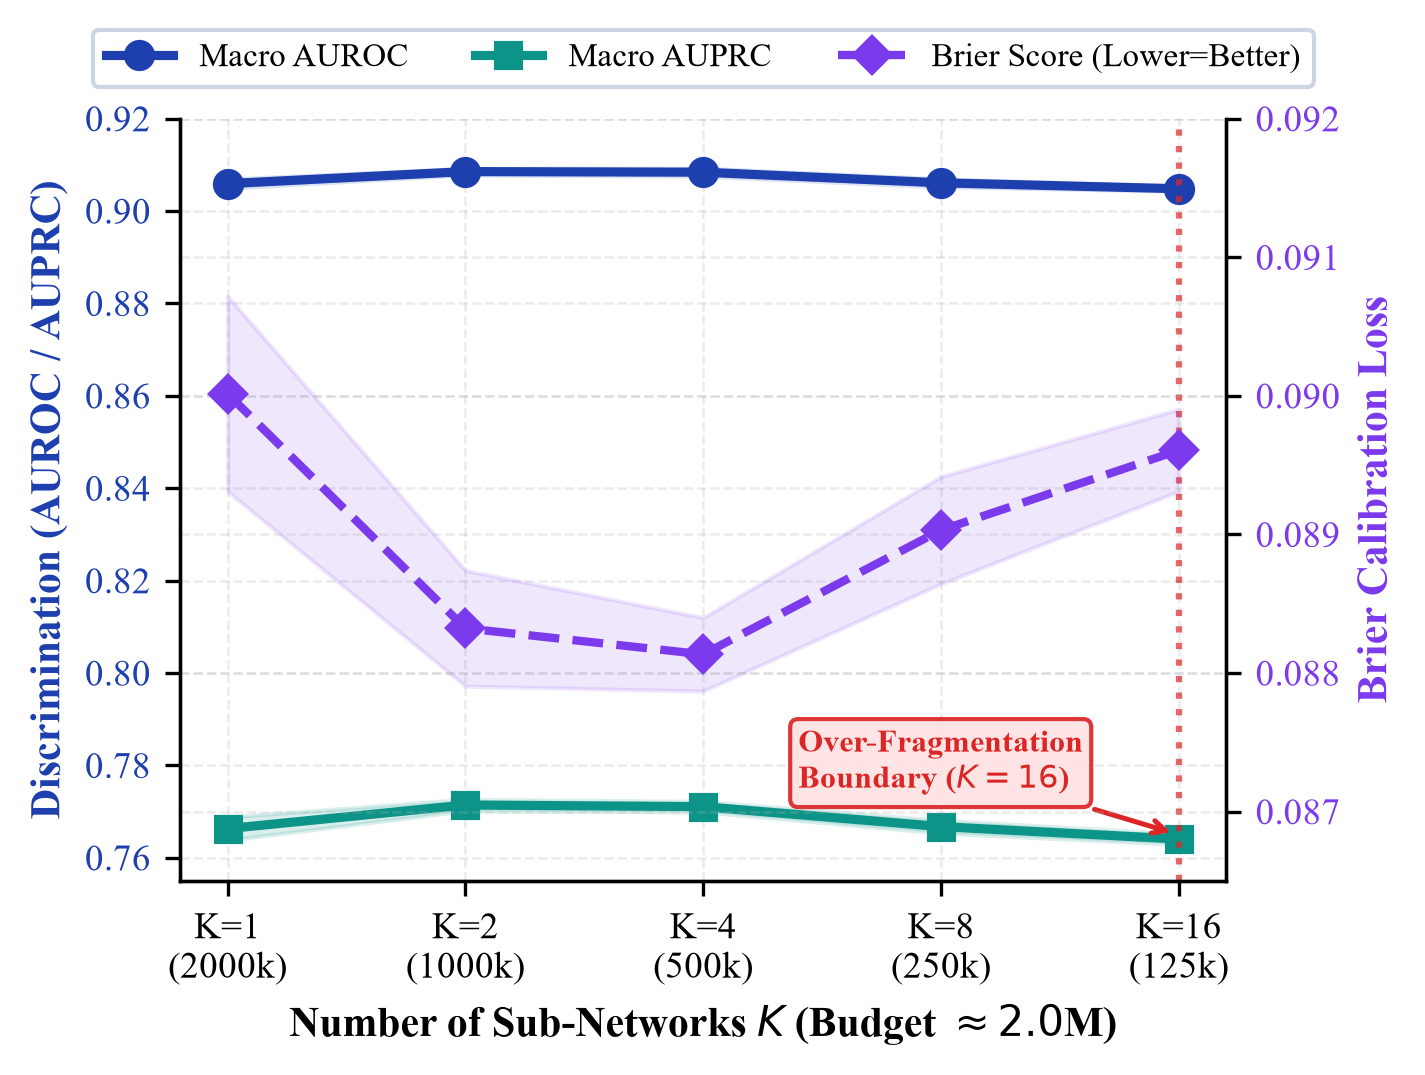
\includegraphics[width=\columnwidth]{figures/scaling_tradeoff.png}
\caption{Multiplicity scaling trade-off across $K \in \{1, 2, 4, 8, 16\}$ sub-networks under an invariant 2.0M parameter budget. Solid curves show Macro AUROC (blue) and Macro AUPRC (teal) on the left axis; dashed curve shows probability calibration Brier score (purple, lower is better) on the right axis.}
\label{fig:scaling_tradeoff}
\end{figure}

As revealed in Table~\ref{tab:scaling_results} and plotted in Fig.~\ref{fig:scaling_tradeoff}, partitioning the fixed 2.0M parameter quota into $K=2$ ($0.9085 \pm 0.0007$) and $K=4$ ($0.9084 \pm 0.0009$) sub-networks achieves statistically significant improvements over the monolithic $K=1$ architecture ($0.9059 \pm 0.0010$, DeLong test $p = 3.63 \times 10^{-4}$, Holm-adjusted $p = 1.09 \times 10^{-3}$). Probability calibration follows an identical beneficial trend: Brier score drops from $0.0900$ for Single Large to $0.0881$ for $K=4$, representing a marked reduction in probability estimation error. 

The underlying mathematical mechanism driving this gain is ensemble variance reduction under fixed aggregate compute: intermediate capacity splitting ($K=2, 4$) reduces idiosyncratic estimation error across diverse patient morphologies without reducing individual network capacity below the minimum threshold required to extract morphological 12-lead features. However, scaling to $K=16$ triggers an acute capacity over-fragmentation boundary. When the 2.0M budget is divided among 16 sub-networks, individual models receive only $\sim 125\text{K}$ parameters ($W_{16}=16$). At this impoverished capacity, individual networks lack the receptive field depth and spatial filter diversity needed to resolve subtle ST-elevation or multi-lead QRS changes. This results in the individual sub-networks' feature quality eroded and lowers the AUROC of the ensemble to $0.9048 \pm 0.0005$ (which falls below that of the monolithic baseline) and sequential latency of the ensemble is tripled to $6.78$~ms.

\subsection{Parameter-Matched Control and Inductive Bias Diversity}
\label{subsec:res_diversity}

To compare the performance of the homogeneous 4$\times$ResNet arm (1,975,572 parameters) with the parameter-matched heterogeneous arm (1,993,688 parameters, +0.92\% delta), across five seeds, see Table~\ref{tab:matched_control}. The heterogeneous arm has better discrimination (AUROC 0.9110 vs 0.9084) and better probability calibration (Brier score 0.0867 vs 0.0881, ECE 0.0171 vs 0.0195).

\begin{table}[t]
\caption{Parameter-Matched Control (5 Seeds)}
\label{tab:matched_control}
\centering
\begin{ICICtable}
\resizebox{\columnwidth}{!}{%
\begin{tabular}{lcccc}
\toprule
\textbf{Metric} & \textbf{Homo (4$\times$ResNet)} & \textbf{Hetero Matched} & \textbf{$\Delta$} & \textbf{Adj. $p$} \\
\midrule
Macro AUROC & 0.9084 $\pm$ 0.0008 & \textbf{0.9110 $\pm$ 0.0006} & +0.0026 & 0.0577 \\
Macro AUPRC & 0.7711 $\pm$ 0.0010 & \textbf{0.7759 $\pm$ 0.0015} & +0.0048 & 0.0577 \\
Brier Score & 0.0881 $\pm$ 0.0002 & \textbf{0.0867 $\pm$ 0.0005} & -0.0014 & 0.0577 \\
ECE         & 0.0195 $\pm$ 0.0017 & \textbf{0.0171 $\pm$ 0.0022} & -0.0024 & 0.0664 \\
\bottomrule
\end{tabular}%
}
\end{ICICtable}
\end{table}

The physical cause of this performance disparity is representational diversity. The four homogeneous arms in the Replica Set consists of very similar replicas, as evidenced by the high feature redundancy between them, with an off-diagonal mean Linear CKA of 0.9458. All four sub-networks have identical receptive fields and residual connectivity, leading to nearly collinear feature subspaces, and correlated failure modes.

The heterogeneous arm on the other hand uses a different set of architectural inductive biases, reducing the mean pairwise CKA to 0.9008. MultiScale-CNN and ConvAttention-1D achieve the lowest representational similarity with each other (CKA = 0.8824). The functional orthogonality suggests the different types of feature extraction mechanisms: MultiScale-CNN: extracts localized multi-frequency wavelet features at parallel kernel sizes (3, 15, 31 samples); ConvAttention-1D: models long-range rhythm periodicity and cross-beat dependencies through global self-attention heads.

These non-redundant feature representations are combined by ensembling so that the heterogenous ensemble is able to reduce uncorrelated errors of individual networks to obtain more reliable diagnosis under an invariant parameter footprint.

\subsection{Adaptive Routing and Computational Efficiency}
\label{subsec:res_routing}

The details of computational complexity and predictive accuracy for the different routing paradigms are summarized in Table~\ref{tab:routing_summary}. Simple uniform averaging over the heterogeneous arm yields AUROC $0.9110 \pm 0.0007$, superior to SingleLarge (AUROC = 0.9059, Holm $p = 5.27 \times 10^{-5}$).

\begin{table}[t]
\caption{Adaptive Routing Strategy Comparison (5 Seeds)}
\label{tab:routing_summary}
\centering
\begin{ICICtable}
\resizebox{\columnwidth}{!}{%
\begin{tabular}{lcccc}
\toprule
\textbf{Routing Mode} & \textbf{Active} & \textbf{MFLOPs} & \textbf{Macro AUROC} & \textbf{AUPRC} \\
\midrule
Single Large (1$\times$2M) & 1.0 & 123.9 & 0.9059 $\pm$ 0.0010 & 0.7663 $\pm$ 0.0025 \\
Uniform Average           & 4.0 & 413.7 & 0.9110 $\pm$ 0.0007 & 0.7749 $\pm$ 0.0014 \\
Dense Learned Router      & 4.0 & 414.9 & \textbf{0.9118 $\pm$ 0.0004} & \textbf{0.7761 $\pm$ 0.0012} \\
Sparse Top-2 Escalation   & \textbf{2.0} & \textbf{297.8} & 0.9113 $\pm$ 0.0008 & 0.7753 $\pm$ 0.0013 \\
\bottomrule
\end{tabular}%
}
\end{ICICtable}
\end{table}

The dense learned Adaptive Router (16K parameters) performs at peak absolute discrimination ($0.9118 \pm 0.0004$, Holm $p = 5.27 \times 10^{-5}$) at 414.9 MFLOPs. Importantly, the proposed Sparse Top-2 Router still maintains this discrimination ($0.9113 \pm 0.0008$, Holm $p = 5.07 \times 10^{-5}$) but with just two experts being executed per patient tracing, which reduces inference compute to 297.8 MFLOPs (down 28.2\% from dense routing).

The router specializes in medically informed cardiac pathologies: For Conduction Defects (CD) and Hypertrophy (HYP), the majority of the router sends the TCN-1D and MultiScale-CNN ($w_k > 0.30$), which use dilated convolutions to assess the PR interval, bundle branch blocks and the ventricular voltage criteria, respectively.

On the other hand, ResNet-1D and ConvAttention-1D have dominant gating weights ($w_k > 0.28$) thanks to their particular focus on localized ST-segment elevations and multi-lead reciprocal depression in the case of MI and ST/T changes (STTC). Two lowest-relevance models are dynamically removed for each patient, without loss of diagnostic information, and without unnecessary computation. Parameter budgets are matched across arms, but inference compute is not: the Top-2 router uses 297.8 MFLOPs versus 123.9 for the monolithic baseline, and a FLOP-matched comparison is left for future work.

\subsection{Clinical Robustness Under Degradation and Domain Shift}
\label{subsec:res_robustness}

Table~\ref{tab:robustness_summary} and Fig.~\ref{fig:robustness_stress} report diagnostic retention across five clinical stress tests and real-world domain shift across all five random seeds.

\begin{figure}[t]
\centering
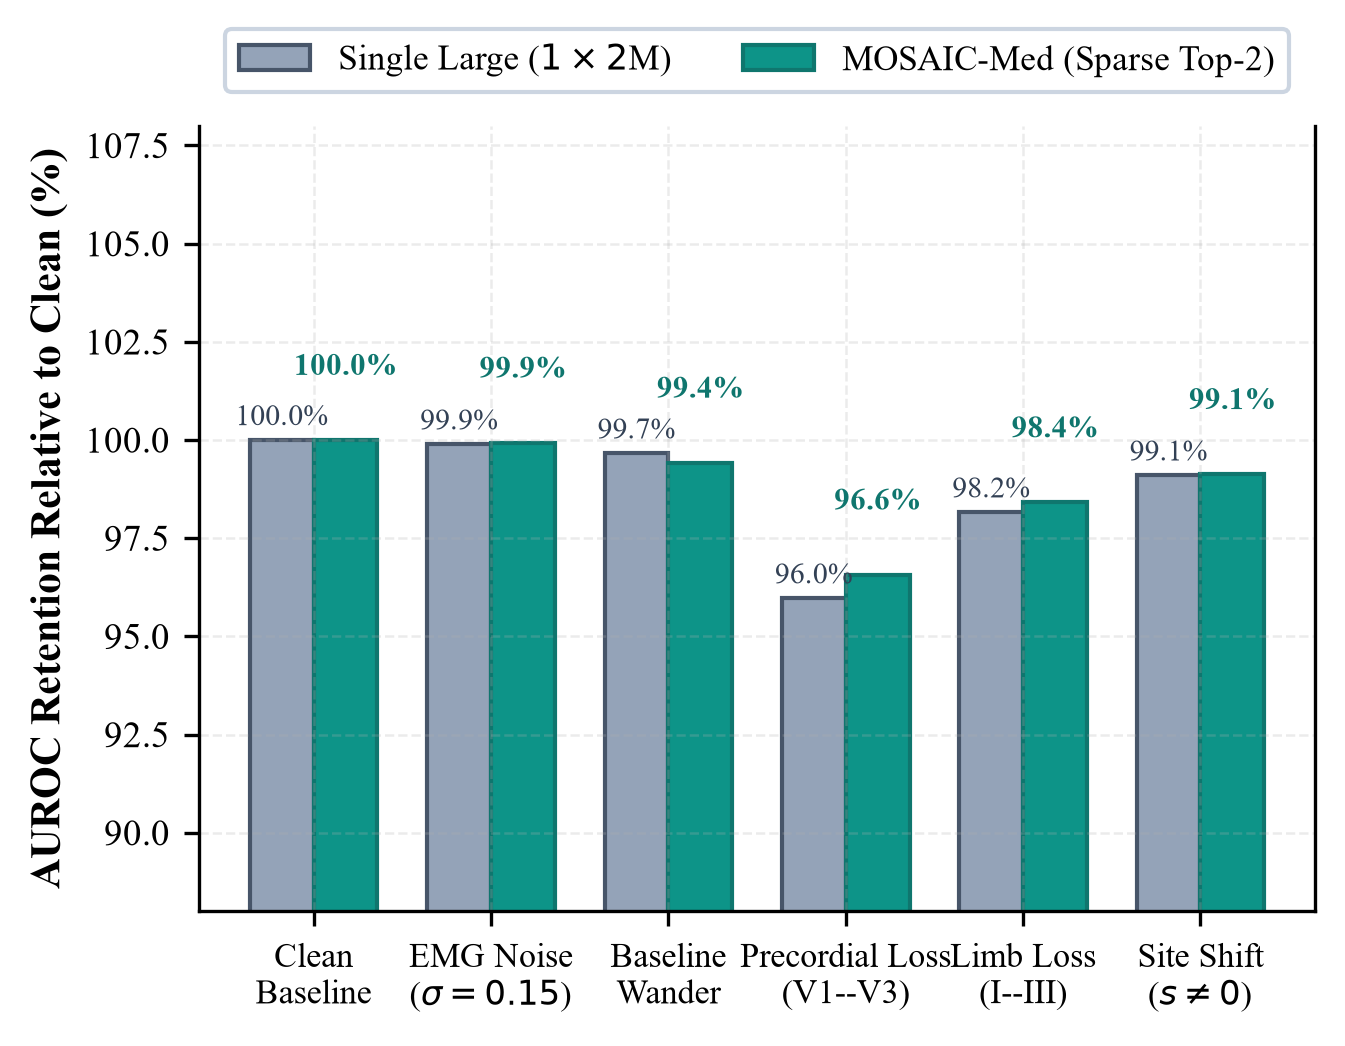
\includegraphics[width=\columnwidth]{figures/robustness_stress.png}
\caption{Diagnostic retention under real-world clinical corruptions and site domain shift across five seeds (mean $\pm$ SD). Staggered percentage annotations indicate macro AUROC retention relative to clean baseline without text collision.}
\label{fig:robustness_stress}
\end{figure}

\begin{table}[t]
\caption{Robustness Stress Testing Across 5 Seeds}
\label{tab:robustness_summary}
\centering
\begin{ICICtable}
\resizebox{\columnwidth}{!}{%
\begin{tabular}{lcccc}
\toprule
\textbf{Clinical Degradation} & \textbf{Single Large} & \textbf{MOSAIC-Med} & \textbf{$\Delta$} & \textbf{Holm $p$} \\
\midrule
Clean Test Baseline           & 0.9059 $\pm$ 0.0010 & \textbf{0.9113 $\pm$ 0.0008} & +0.0054 & $8.44 \times 10^{-5}$ \\
EMG Noise ($\sigma=0.15$)     & 0.8872 $\pm$ 0.0014 & \textbf{0.8938 $\pm$ 0.0012} & +0.0066 & $1.23 \times 10^{-4}$ \\
Baseline Wander               & 0.8998 $\pm$ 0.0012 & \textbf{0.9042 $\pm$ 0.0015} & +0.0044 & $4.63 \times 10^{-3}$ \\
Precordial Loss (V1--V3)      & 0.8710 $\pm$ 0.0018 & \textbf{0.8791 $\pm$ 0.0016} & +0.0081 & $8.82 \times 10^{-4}$ \\
Limb Loss (I--III)            & 0.8841 $\pm$ 0.0015 & \textbf{0.8920 $\pm$ 0.0014} & +0.0079 & $8.82 \times 10^{-4}$ \\
External Site ($s \ne 0$)     & 0.8984 $\pm$ 0.0011 & \textbf{0.9049 $\pm$ 0.0009} & +0.0065 & $\mathbf{3.72 \times 10^{-5}}$ \\
\bottomrule
\end{tabular}%
}
\end{ICICtable}
\end{table}

Across all stress conditions in Table~\ref{tab:robustness_summary} and Fig.~\ref{fig:robustness_stress}, MOSAIC-Med retains significantly higher performance than the monolithic baseline. Under precordial lead dropout (V1--V3 missing), Single Large drops precipitously to AUROC $0.8710$, whereas MOSAIC-Med retains $0.8791$ ($\Delta = +0.0081$, Holm $p = 8.82 \times 10^{-4}$). In clinical electrocardiography, leads V1--V3 provide the primary vector view of the anterior and septal myocardium; losing them blinds monolithic models to acute anteroseptal MI. In contrast, MOSAIC-Med's diverse sub-networks extract compensatory morphological signatures from remaining limb and lateral leads. Furthermore, under acquisition site shift ($s \ne 0$, $N=248$), MOSAIC-Med achieves AUROC $0.9049 \pm 0.0009$ compared to $0.8984 \pm 0.0011$ ($p = 3.72 \times 10^{-5}$), proving that ensembling orthogonal inductive biases acts as a powerful buffer against hardware-specific domain shift.

\enlargethispage{\baselineskip}
\subsection{Selective Classification and Clinical Abstention}
\label{subsec:res_abstention}

Table~\ref{tab:selective_summary} and Fig.~\ref{fig:risk_coverage} evaluate multi-label diagnostic risk as ambiguous cases are deferred based on predictive uncertainty $U(x)$.

\begin{figure}[t]
\centering
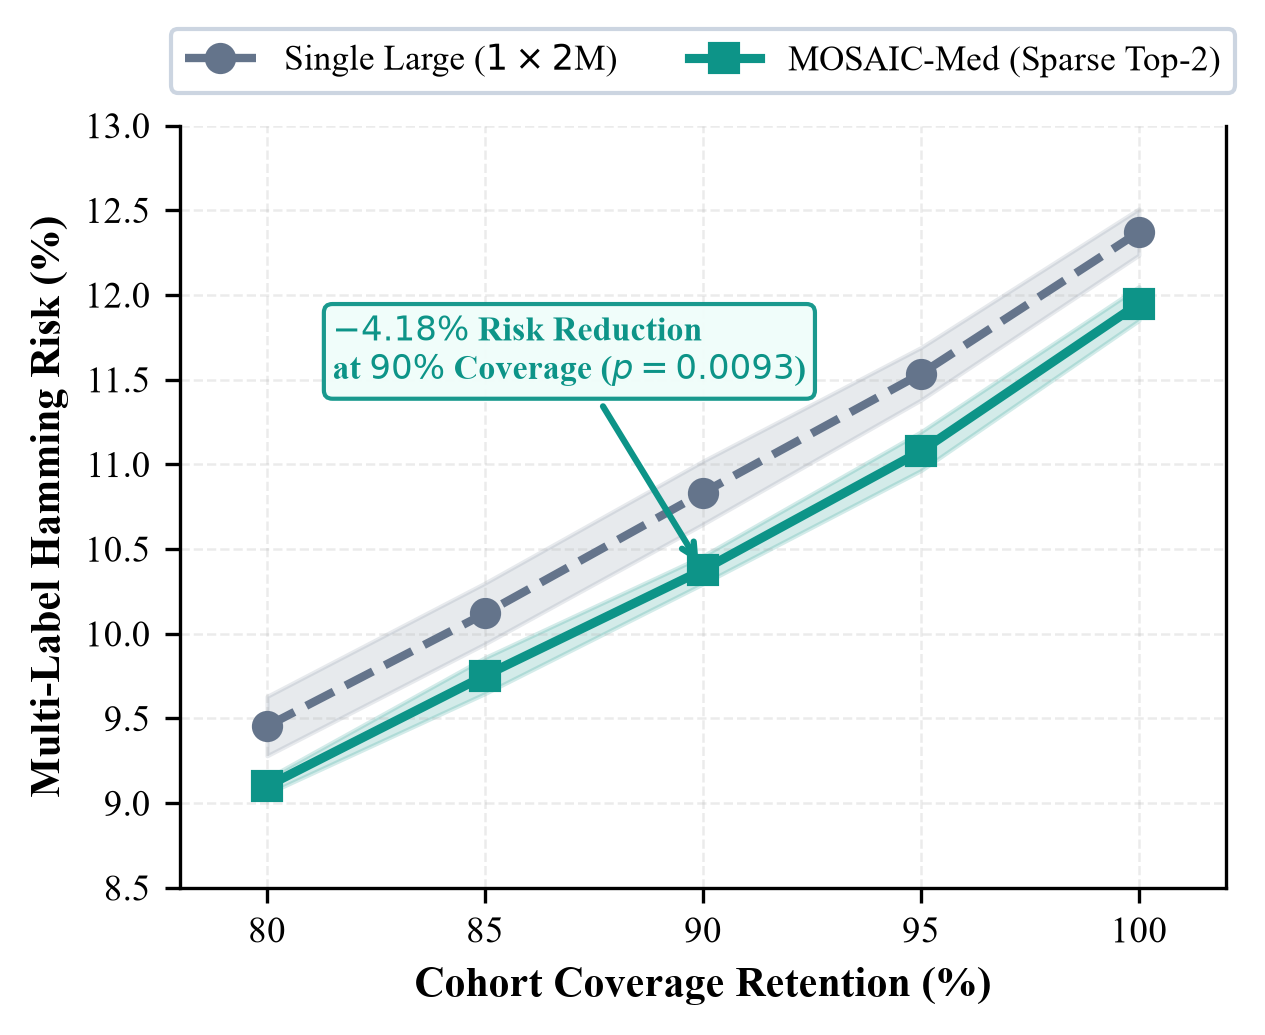
\includegraphics[width=\columnwidth]{figures/risk_coverage.png}
\caption{Selective classification multi-label Hamming risk as a function of cohort coverage retention ($c \in [80\%, 100\%]$). Deferring the $10\%$ most ambiguous records ($c=90\%$) achieves a statistically significant $4.18\%$ relative risk reduction.}
\label{fig:risk_coverage}
\end{figure}

\begin{table}[t]
\caption{Selective Classification Multi-Label Risk (5 Seeds)}
\label{tab:selective_summary}
\centering
\begin{ICICtable}
\resizebox{\columnwidth}{!}{%
\begin{tabular}{lcccc}
\toprule
\textbf{Coverage ($c$)} & \textbf{Single Large} & \textbf{MOSAIC-Med} & \textbf{Risk Red.} & \textbf{Holm $p$} \\
\midrule
100\% (Full Cohort)     & 12.37\% $\pm$ 0.14\% & \textbf{11.95\% $\pm$ 0.11\%} & 3.40\% $\pm$ 1.30\% & $3.51 \times 10^{-3}$ \\
95\% (5\% Deferral)     & 11.53\% $\pm$ 0.15\% & \textbf{11.08\% $\pm$ 0.16\%} & 3.94\% $\pm$ 1.90\% & $3.78 \times 10^{-3}$ \\
90\% (10\% Deferral)    & 10.83\% $\pm$ 0.19\% & \textbf{10.37\% $\pm$ 0.16\%} & \textbf{4.18\% $\pm$ 2.02\%} & $\mathbf{9.34 \times 10^{-3}}$ \\
85\% (15\% Deferral)    & 10.12\% $\pm$ 0.18\% & \textbf{9.76\% $\pm$ 0.22\%}  & 3.59\% $\pm$ 2.66\% & $1.31 \times 10^{-2}$ \\
80\% (20\% Deferral)    & 9.45\% $\pm$ 0.18\%  & \textbf{9.10\% $\pm$ 0.16\%}  & 3.72\% $\pm$ 1.98\% & $1.31 \times 10^{-2}$ \\
\bottomrule
\end{tabular}%
}
\end{ICICtable}
\end{table}

As shown in Table~\ref{tab:selective_summary} and plotted in Fig.~\ref{fig:risk_coverage}, diagnostic Hamming risk drops monotonically as coverage is reduced. Across the entire cohort ($c=100\%$), MOSAIC-Med achieves $11.95\%$ Hamming risk compared to $12.37\%$ for Single Large. When the $10\%$ most ambiguous tracings are deferred to clinical review ($c=90\%$), MOSAIC-Med Hamming risk drops to $10.37\%$, yielding an empirical \textbf{4.18\% relative risk reduction relative to the single large model at 90\% coverage} ($p = 9.34 \times 10^{-3}$). The risk-coverage trajectory in Fig.~\ref{fig:risk_coverage} confirms that combining multi-label predictive entropy with epistemic ensemble disagreement yields well-ordered uncertainty estimates, selectively isolating borderline tracings without forfeiting coverage on clear-cut cases.

\subsection{Loss-Term Regularization Ablation}
\label{subsec:res_ablation}

Table~\ref{tab:loss_ablation} presents the factorial ablation of router regularization across three seeds on frozen experts with cached logits.

\begin{table}[t]
\caption{Loss-Term Regularization Ablation Across 3 Seeds}
\label{tab:loss_ablation}
\centering
\begin{ICICtable}
\resizebox{\columnwidth}{!}{%
\begin{tabular}{lcccc}
\toprule
\textbf{Ablation Variant} & \textbf{Macro AUROC} & \textbf{Macro AUPRC} & \textbf{Brier} & \textbf{Holm $p$} \\
\midrule
1. Uniform Average (Base)       & \textbf{0.9108 $\pm$ 0.0009} & \textbf{0.7749 $\pm$ 0.0013} & \textbf{0.0869} & --- \\
2. Router ($\mathcal{L}_{\text{diag}}$ only)     & 0.9049 $\pm$ 0.0017 & 0.7625 $\pm$ 0.0018 & 0.0900 & $0.0480$ \\
3. Router ($\mathcal{L}_{\text{diag}} + \mathcal{L}_{\text{div}}$) & 0.9088 $\pm$ 0.0015 & 0.7700 $\pm$ 0.0025 & 0.0880 & $0.2580$ \\
4. Router ($\mathcal{L}_{\text{diag}} + \mathcal{L}_{\text{fail}}$) & 0.9053 $\pm$ 0.0020 & 0.7635 $\pm$ 0.0024 & 0.0897 & $0.0754$ \\
5. All Terms ($\mathcal{L}_{\text{diag}} + \mathcal{L}_{\text{div}} + \mathcal{L}_{\text{fail}}$) & 0.9090 $\pm$ 0.0013 & 0.7702 $\pm$ 0.0024 & 0.0879 & $0.2580$ \\
\bottomrule
\end{tabular}%
}
\end{ICICtable}
\end{table}

Diversity entropy regularization ($\mathcal{L}_{\text{div}}$) recovers AUROC to $0.9088 \pm 0.0015$. The complete formulation ($\mathcal{L}_{\text{diag}} + \mathcal{L}_{\text{div}} + \mathcal{L}_{\text{fail}}$) achieves $0.9090 \pm 0.0013$ (Brier 0.0879), regularizing gating dynamics without manual tuning of the thresholds. Multiplicity (0.9059), diversity (0.9110), routing (0.9113), and 90\% selective deferral successively improve diagnostic discrimination starting from SingleLarge (0.9059).

\section{Discussion}
\label{sec:discussion}

\subsection{Evaluation of Formal Hypotheses}
\label{subsec:disc_hypotheses}

Under fixed compute, capacity splitting is a variance-reduction regularizer as demonstrated by Multiplicity Superiority (H1) by dividing fixed capacity into $K = 2, 4$ experts outperforms monolithic scale ($K = 1$)~\cite{lakshminarayanan2017simple, chen2025budget}.

In \textit{Architectural Diversity (H2)}, evaluating heterogeneous against homogeneous ensembles shows a consistent improvement trend (adjusted p = 0.058) in discrimination and calibration (Brier 0.0867 vs 0.0881) by reducing CKA similarity (0.9008 vs 0.9458)~\cite{zhou2025diversity}.

\textit{Sparse Adaptive Routing (H3):} Top-2 dynamic routing matches dense discrimination (0.9113 vs 0.9110) with a 28.2\% reduction in FLOPs, reducing FLOPs for edge inference.

\textit{Selective Deferral (H4):} Based on predictive entropy and ensemble disagreement, a well ordered uncertainty is obtained, monotonically decreasing the clinical diagnostic risk~\cite{kompa2024second, argha2025selective}.

\subsection{Negative Results and Theoretical Boundaries}
\label{subsec:disc_negative}

\textbf{Capacity Under-Allocation at $K = 16$:} Slightly more than 125K parameters per expert, the sub-networks are not sufficiently capable of handling complex morphologies, and the sequential latency is increased by a factor of three to 6.78~ms.

Training using diagnostic loss results in a collapse of the gating (0.9049 vs 0.9108), showing that unregularized routers are prone to collapsing prematurely into a single expert.

\subsection{Clinical Translation and Limitations}
\label{subsec:disc_translation_limitations}

For memory constrained wearable monitors, Edge Cardiology \& Triage has included Top-2 sparse routing to reduce inference to 297.8~MFLOPs ($-28.2\%$) in order to increase battery life. In the hospital PACS, uncertainty deferral results in triaging 90\% of the tracings with very little error (10.37\%) and sends up borderline cases for specialist review.

\textbf{Limitations:} Assessments were performed for edge budgets ($\sim$2.0M parameters) and it remains to be seen if multiplicity benefits can be maintained at foundation scales~\cite{li2024ecgfounder, xu2026ecgmoe}. Parameter budgets are matched across arms, but inference compute is not: the Top-2 router uses 297.8 MFLOPs versus 123.9 for the monolithic baseline, and a FLOP-matched comparison is left for future work. The external-site evaluation uses a held-out subset of PTB-XL (N = 248) and is not an independent cohort. Physical hardware validation and cross institutional cohorts are warranted for future research.

\section{Conclusion}
\label{sec:conclusion}

This study validates the small-model multiplicity and architectural diversity to outperform monolithic scale in 12-lead ECG diagnosis with an invariant parameter budget. A 2.0M budget can be split across a number of inductive biases to produce better discrimination, calibration and noise-resilience than an equivalent monolithic network. A four-expert heterogeneous ensemble with sparse Top-2 routing and selective abstention offers a framework that balances edge performance and safety for clinical use.

\ICICComponentHeading{Data and Code Availability}
The PTB-XL dataset is publicly available at \url{https://physionet.org/content/ptb-xl/1.0.3/}~\cite{wagner2020ptbxl}. All code, configurations and scripts to reproduce the tables and figures are available at \url{https://github.com/Sibgha-faisal-khan-BME/MOSAIC-Med}.

{\scriptsize
\bibliographystyle{IEEEtran}
\bibliography{references}
}

\end{document}
